\documentclass[6008notes.tex]{subfiles}
\begin{document}
\graphicspath{ {images/indepstruct/} }

\section{Independence Structure}

\subsection{Independent Events}

When you flip a coin or roll dice, the outcome of a coin flip or a die roll isn't going to tell you anything about the outcome of a new coin toss or die roll unless you have some very peculiar coins or dice.

we're going to formalize this by saying that two events A and B are independent, which we'll denote by this thing that looks like an upside down T: $\bigCI$

{\centering $A \bigCI B \qquad \text{if} \qquad \mathbb {P}(A \cap B) = \mathbb {P}(A) \mathbb {P}(B)$ \par}

If $\mathbb {P}(A) > 0$ we can use the product rule for events to rewrite the left side:

{\centering $\mathbb {P}(B \mid A) \mathbb {P}(A) = \mathbb {P}(A) \mathbb {P}(B)$ \par}

Cancelling $\mathbb {P}(A)$ on both sides:

{\centering $A \bigCI B \qquad \text{if} \qquad \mathbb {P}(B \mid A) = \mathbb {P}(B)$ \par}

Similarly, if $\mathbb {P}(B) > 0$

{\centering $A \bigCI B \qquad \text{if} \qquad \mathbb {P}(A \mid B) = \mathbb {P}(A)$ \par}

So knowing $B$ doesn't tell us anything new about $A$, and \textit{vice versa}.

\subsection{Independent Random Variables}

$X$ and $Y$ are independent ($X \bigCI Y$) if $p_{X,Y} (x,y) = p_X(x)p_Y(y)$.

Knowing one gives no information about the other, so $p_{X \mid Y} (x \mid y) = p_X(x)$.

\paragraph{Exercise: Independent Random Variables}  In this exercise, we look at how to check if two random variables are independent in Python. Please make sure that you can follow the math for what's going on and be able to do this by hand as well.

Consider random variables $W$, $I$, $X$, and $Y$, where we have shown the joint probability tables $p_{W,I}$ and $p_{X,Y}$.

{\centering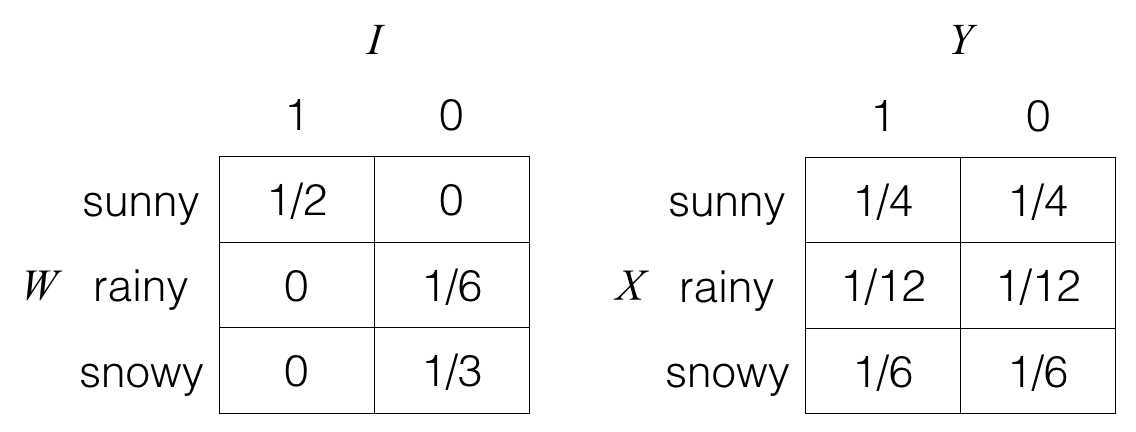
\includegraphics[scale=0.4]{images_sec-joint-rv-ex-marg} \par}

In Python:

\begin{lstlisting}
prob_W_I = np.array([[1/2, 0], [0, 1/6], [0, 1/3]])
\end{lstlisting}

Note that here, we are not explicitly storing the labels, but we'll keep track of them in our heads. The labels for the rows (in order of row index): sunny, rainy, snowy. The labels for the columns (in order of column index): 1, 0.

We can get the marginal distributions $p_W$ and $p_I$:

\begin{lstlisting}
prob_W = prob_W_I.sum(axis=1)
prob_I = prob_W_I.sum(axis=0)
\end{lstlisting}

Then if $W$ and $I$ were actually independent, then just from their marginal distributions $p_W$ and $p_I$, we would be able to compute the joint distribution with the formula:

{\centering$\text {If $W$ and $I$ are independent:} \qquad p_{W,I}(w,i)=p_ W(w)p_ I(i) \qquad \text {for all }w,i.$ \par}
 
Note that variables \lstinline{prob_W} and \lstinline{prob_I} at this point store the probability tables $p_W$ and $p_I$ as 1D NumPy arrays, for which NumPy does \textit{not} store whether each of these should be represented as a row or as a column.

We could however ask NumPy to treat them as column vectors, and in particular, taking the outer product of \lstinline{prob_W} and \lstinline{prob_I} yields what the joint distribution would be if $W$ and $I$ were independent:

\begin{eqnarray*}
\begin{bmatrix}
p_W(\text{sunny}) \\
p_W(\text{rainy}) \\
p_W(\text{snowy})
\end{bmatrix}
\begin{bmatrix}
p_I(1) & p_I(0)
\end{bmatrix}
=
\begin{bmatrix}
p_W(\text{sunny})p_I(1) & p_W(\text{sunny})p_I(0) \\
p_W(\text{rainy})p_I(1) & p_W(\text{rainy})p_I(0) \\
p_W(\text{snowy})p_I(1) & p_W(\text{snowy})p_I(0)
\end{bmatrix}.
\end{eqnarray*}

The left-hand side is an outer product, and the right-hand side is precisely the joint probability table that would result if $W$ and $I$ were independent.

To compute and print the right-hand side, we do:

\begin{lstlisting}
print(np.outer(prob_W, prob_I))
\end{lstlisting}

TODO - add notes from video

\subsection{Practice Problem: Conditional Independence}

Suppose $X_0, \dots , X_{100}$ are random variables whose joint distribution has the following factorization:

{\centering$p_{X_0, \dots , X_{100}}(x_0, \dots , x_{100}) = p_{X_0}(x_0) \cdot \prod _{i=1}^{100} p_{X_ i | X_{i-1}}(x_ i | x_{i-1})$ \par}
 
This factorization is what's called a Markov chain. We'll be seeing Markov chains a lot more later on in the course.

Show that $X_{50} \perp X_{52} | X_{51}$.

Solution: Notice that we can marginalize out $x_{100}$ as such:

{\centering$p_{X_0, \dots , X_{99}}(x_0, \dots , x_{99}) = p_{X_0}(x_0) \cdot \prod _{i=1}^{99} p_{X_ i | X_{i-1}}(x_ i | x_{i-1}) \cdot \underbrace{\sum _{x_{100}} p_{X_{100}|X_{99}}(x_{100}|x_{99})}_{= 1} \qquad\qquad$ (2.5) \par}
 
Now we can repeat the same marginalization procedure to get:

{\centering$p_{X_0, \dots , X_{50}}(x_0, \dots , x_{50}) = p_{X_0}(x_0) \cdot \prod _{i=1}^{50} p_{X_ i | X_{i-1}}(x_ i | x_{i-1})$ \par}

In essence, we have shown that the given joint distribution factorization applies not just to the last random variable ($X_{100}$), but also up to any point in the chain.

For brevity, we will now use $p(x_{i}^{j})$ as a shorthand for $p_{X_ i, \dots , X_{j}}(x_ i, \dots , x_{j})$. We want to exploit what we have shown to rewrite $p(x_{50}^{52})$

\begin{eqnarray*}
		p(x_{50}^{52})
        &=& \sum_{x_{0} \dots x_{49}} \sum_{x_{53} \dots x_{100}} p(x_{0}^{100}) \\
		&=& \sum_{x_{0} \dots x_{49}} \sum_{x_{53} \dots x_{100}} \left[p(x_{0}) \prod_{i=0}^{50} p(x_{i}|x_{i-1})\right] \cdot p(x_{51}|x_{50}) \cdot p(x_{52}|x_{51}) \cdot \prod_{i=53}^{100} p(x_{i}|x_{i-1}) \\
		&=& \sum_{x_{0} \dots x_{49}} \sum_{x_{53} \dots x_{100}} p(x_{0}^{50}) \cdot p(x_{51}|x_{50}) \cdot p(x_{52}|x_{51}) \cdot \prod_{i=53}^{100} p(x_{i}|x_{i-1}) \\
		&=& p(x_{51}|x_{50}) \cdot p(x_{52}|x_{51}) \cdot \sum_{x_{0} \dots x_{49}} p(x_{0}^{50}) \underbrace{\sum_{x_{53} \dots x_{100}} \prod_{i=53}^{100} p(x_{i}|x_{i-1})}_{=1} \\
		&=& p(x_{51}|x_{50}) \cdot p(x_{52}|x_{51}) \cdot \sum_{x_{0} \dots x_{49}} p(x_{0}^{50}) \\
		&=& p(x_{50}) \cdot p(x_{51}|x_{50}) \cdot p(x_{52}|x_{51})
    \end{eqnarray*}
		
where we used (2.5) for the 3rd equality and the same marginalization trick for the 5th equality. We have just shown the Markov chain property, so the conditional independence property must be satisfied.

\subsection{Mutual vs Pairwise Independence}

To extend the independence story to more than two variables, the strongest way is by using something called ``mutual independence''. We'll say that three random variables  $X$, $Y$, and $Z$ are mutually independent if we can write  the joint distribution as simply the product of the three individual distributions:

{\centering$p_{X,Y,Z} (x,y,z) = p_X(x) p_Y(y) p_Z(z)$ \par}

Knowing $X$ and $Y$ won't tell you anything about $Z$. Knowing $X$ won't tell you anything about $Y$. They're completely independent.

There are also weaker forms of independence that we're interested in, for example, ``pairwise independence''. This means that for any two variables, you can write:

{\centering$p_{X,Y} (x,y) = p_X(x) p_Y(y)$ \par}

and similarly for $Y,Z$ and $X,Z$. This is saying if I know any one, it doesn't tell me think anything about any of the others. But this is not the same as mutual independence, it's not as strong.

As an example of why, suppose that we have two random variables $X$ and $Y$. They both represent independent fair coin flips. We'll write the outcomes as 0 and 1, and each one has a 50-50 chance of being heads or tails, 0 or 1.

We'll define $Z = X \oplus Y$, where ``XOR'' (written $\oplus$) is defined to be a function that takes in two things and returns 1 when exactly one of them is 1:

\begin{center}
\begin{tabular}{| c | c | c }
\textbf{x} & \textbf{y} & \textbf{z} \\
\hline
0 &	0 &	0 \\
0 &	1 &	1 \\
1 &	0 &	1 \\
1 &	1 &	0 \\
\end{tabular}
\end{center}

What's the probability $p_{X,Y}$ for each of these configurations? They're independent fair coin flips, so each is equally likely. The probability of any particular one is 0.5 for $X$ times 0.5 for $Y$, so 0.25:

\begin{center}
\begin{tabular}{| c | c | c | c }
$\mathbf{p_{X,Y}}$ & \textbf{x} & \textbf{y} & \textbf{z} \\
\hline
0.25 & 0 &	0 &	0 \\
0.25 & 0 &	1 &	1 \\
0.25 & 1 &	0 &	1 \\
0.25 & 1 &	1 &	0 \\
\end{tabular}
\end{center}

What's the distribution for Z? There are two ways to get $z=0$ and they each have probability 0.25. If we add them up then we have a 0.5 chance of $z$ being 0 and similarly a 0.5 chance of $z$ being 1. 

\begin{eqnarray*}
p_Z(z)
&=&
\begin{cases}
  0.5 & \text{if }z=0 \\
  0.5 & \text{if }z=1
\end{cases}
\end{eqnarray*}

What's $Z$ given $X$? Well, it's actually the same. If $x=0$, then we can restrict ourselves to just looking at the top two rows of the table, so Z can either be 0 or 1. And, again, they're equally likely so it's 50-50. If $x=1$, we can just look at the bottom two rows, and again they're equally likely, 50-50. 

\begin{eqnarray*}
p_{Z \mid X}(z \mid x)
&=&
\begin{cases}
  0.5 & \text{if }z=0 \\
  0.5 & \text{if }z=1
\end{cases}
\end{eqnarray*}

So $p_{Z \mid X}(z \mid x) = p_Z(z)$, it doesn't depend on X at all. So this means that $Z \bigCI X$.

By symmetry, we can make the same argument for $Z \bigCI Y$, and we said at the start that $X \bigCI Y$. So here we have three random variables that are all pairwise independent --- if you look at any pair, knowing one doesn't tell you about the other. 

But if we look all together, they're not mutually independent. For example, if I know any two of them, then I know exactly what the third one is going to be. The distribution over the third one changes from being fair 50-50 to being deterministic. For example, if $X$ is 0 and $Y$ is 0, then $Z$ is also going to be 0. And if I didn't know that, then the probability would be 50-50. Once I do know that, the probability becomes 1 that it's 0 and 0 that it's anything else. So here, they're not mutually independent. In this example it may seem a little contrived, but in general, it's often tempting to assume that knowing things are pairwise independent tells you that they're mutually independent. But you have to be aware that they're not.

\subsection{Conditional Independence}

TODO - add notes from video


\end{document}